\documentclass[12pt]{article}
\usepackage{listings}
\usepackage{color}
\usepackage{graphicx}
\usepackage{subcaption}
\usepackage{caption}
\usepackage[a4paper]{geometry}
\usepackage{wrapfig}
\usepackage{lscape}
\usepackage{rotating}
\usepackage{epstopdf}
\usepackage{url}

\lstset{language=C,
	captionpos=b,
	frame=single,
	breaklines=true,
	basicstyle=\ttfamily,
    keywordstyle=\color{blue}\ttfamily,
    stringstyle=\color{red}\ttfamily,
    commentstyle=\color{green}\ttfamily,
    morecomment=[l][\color{magenta}]{\#}
} 
\renewcommand{\lstlistingname}{Code Snippet} 

\begin{document}

\begin{titlepage}
\newgeometry{bottom=1cm}
\newcommand{\HRule}{\rule{\linewidth}{0.5mm}} % Defines a new command for the horizontal lines, change thickness here
\center % Center everything on the page

%----------------------------------------------------------------------------------------
%	LOGO SECTION
%----------------------------------------------------------------------------------------
\graphicspath{{figures/}}


\includegraphics[width=10cm]{Lboro_Logo.jpg}\\ % Include a department/university logo - this will require 	the graphicx package
 
 \vspace{1cm}

%----------------------------------------------------------------------------------------
%	TITLE SECTION
%----------------------------------------------------------------------------------------

\HRule \\[0.4cm]
{ \huge \bfseries E-Puck Behaviour Implementation}\\[0.4cm] % Title of your document
\HRule \\[1cm]

%----------------------------------------------------------------------------------------
%	HEADING SECTIONS
%----------------------------------------------------------------------------------------

% \textsc{\LARGE Loughborough University}\\[1.5cm] % Name of your university/college

%----------------------------------------------------------------------------------------
\textsc{\Large Robotics and Intelligent Systems}\\[0.5cm] % Major heading such as course name
\textsc{\large COP518}\\[0.5cm] % Minor heading such as course title

 
%----------------------------------------------------------------------------------------
%	AUTHOR SECTION
%----------------------------------------------------------------------------------------

\begin{minipage}{0.4\textwidth}
\begin{flushleft} \large
\emph{Authors:}\\
Ross \textsc{McQuillan}\\
Amr \textsc{Yousef}\\
Xinyu \textsc{Chen}
\end{flushleft}
\end{minipage}
~
\begin{minipage}{0.4\textwidth}
\begin{flushright} \large
\emph{Supervisor:} \\
Dr. Qinggang \textsc{Meng} % Supervisor's Name
\end{flushright}
\end{minipage}\\[2cm]

% If you don't want a supervisor, uncomment the two lines below and remove the section above
%\Large \emph{Author:}\\
%John \textsc{Smith}\\[3cm] % Your name

\vfill % Fill the rest of the page with whitespace

%----------------------------------------------------------------------------------------
%	DATE SECTION
%----------------------------------------------------------------------------------------

{\large \today}\\[2cm] % Date, change the \today to a set date if you want to be precise
\restoregeometry
\end{titlepage}

\newgeometry{bottom=3cm}
\newgeometry{top=2cm}
\tableofcontents
\clearpage 
\newgeometry{top=3cm}

\section{Introduction} \label{sec:intro}
Within the Robotics and Intelligence systems module groups worked together to implement different behaviours with an E-Puck. Many different behaviours were available for implementation, including attraction, hate and aggression.

This report will explain, in detail, the tasks set out before each group. It will progress by explaining the design established to tackle these objectives, the implementation of the design, testing and results before concluding the coursework and evaluating the groups achievements.

The tasks given to each group were split into two separate parts. The first was to develop a behaviour on a single E-Puck. Such initial behaviours proposed by Dr. Meng, included love where the E-Puck would follow close to, but without touching, an object or, obstacle avoidance, where the E-Puck would try to avoid objects. More of the behaviours will be spoken about throughout this report in greater detail.

The second task included using two E-Pucks. One of the E-Pucks was tasked with following a human hand but not other objects, whilst the other was to follow the first E-Puck closely without touching it. This second E-Puck would imitate the love behaviour spoken about previously.
\section{Background} \label{sec:background}
The robotics industries association\cite{RIA} defines a robot ``a re-programmable, multi-functional, manipulator designed to move material, parts, tools or specialised devices through variable programmed motions for the performance of a variety of task''\cite{RIAdefinition}. According to that definition any device that is programmed to preform variety of tasks is classified as a robot. Most robots consist of several hardware components such as:
\begin{itemize}
	\item Physical body
	\item Actuators
	\item Sensors
	\item Controller
	\item Processor
	\item Software 
\end{itemize}
These components are commonly used when designing and developing a robot. A good design is considered to be one which best utilizes these components to reach it's goals effectively and efficiently.
\subsection{Behaviours}
Many different behaviours can be seen in day to day life. If one was trying to describe a behaviour as simply as possible, one might say a behaviour is a ``mapping of sensory inputs to a pattern of motor actions that are used to achieve a task''\cite{BehaviourDef}. The behaviours robots wish to imitate include all of the common human behaviours. Getting the robots to show a very basic version of this behaviour, such as love, would require the robot to follow nearby object in a show of attraction. Naturally, the main goal in cutting edge research is to develop these skills such that they are indistinguishable to the fully fletched human behaviours.

\subsection{E-Puck}

\begin{figure}
\centering
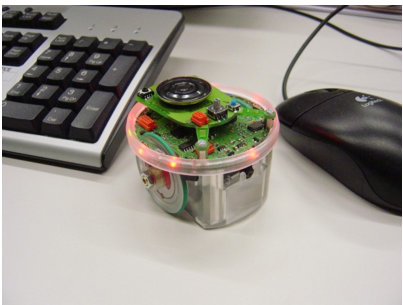
\includegraphics[width=0.7\linewidth]{figures/epcuk}
\caption{}
\label{fig:epcuk}
\end{figure}


An E-Puck\cite{epuck} is a small sized, educational robot which is designed to allow developers to code on and learn about robotics. The robot is very inexpensive, user-friendly and interactive. It was designed by Martin Stefanec from the artificial life lab of University of Graz who made all the software developed for the E-Puck open source.

It includes a wide range of sensors and actuators. Sensors include infrared-sensors which can be used to detect objects and ambient light, motors to control the movement of the robot and for communication the robot is has 8 LEDs, a speaker and bluetooth.

\subsection{HSV}

HSV stands for Hue, Saturation and value. It's a cylindrical representation of colours, starting at red in 0 degrees, green at 120 degrees and blue at 240 degrees. Using figure \ref{fig:hsv} one can recognise that the colour space's saturation is most intense in the centre of the cylinder. The saturation decides how washed out the colours appear. The final component value, which increases the higher up the cylinder the pixel value is, decides how much colour or how vibrant each colour appears.

\begin{figure}
	\centering
	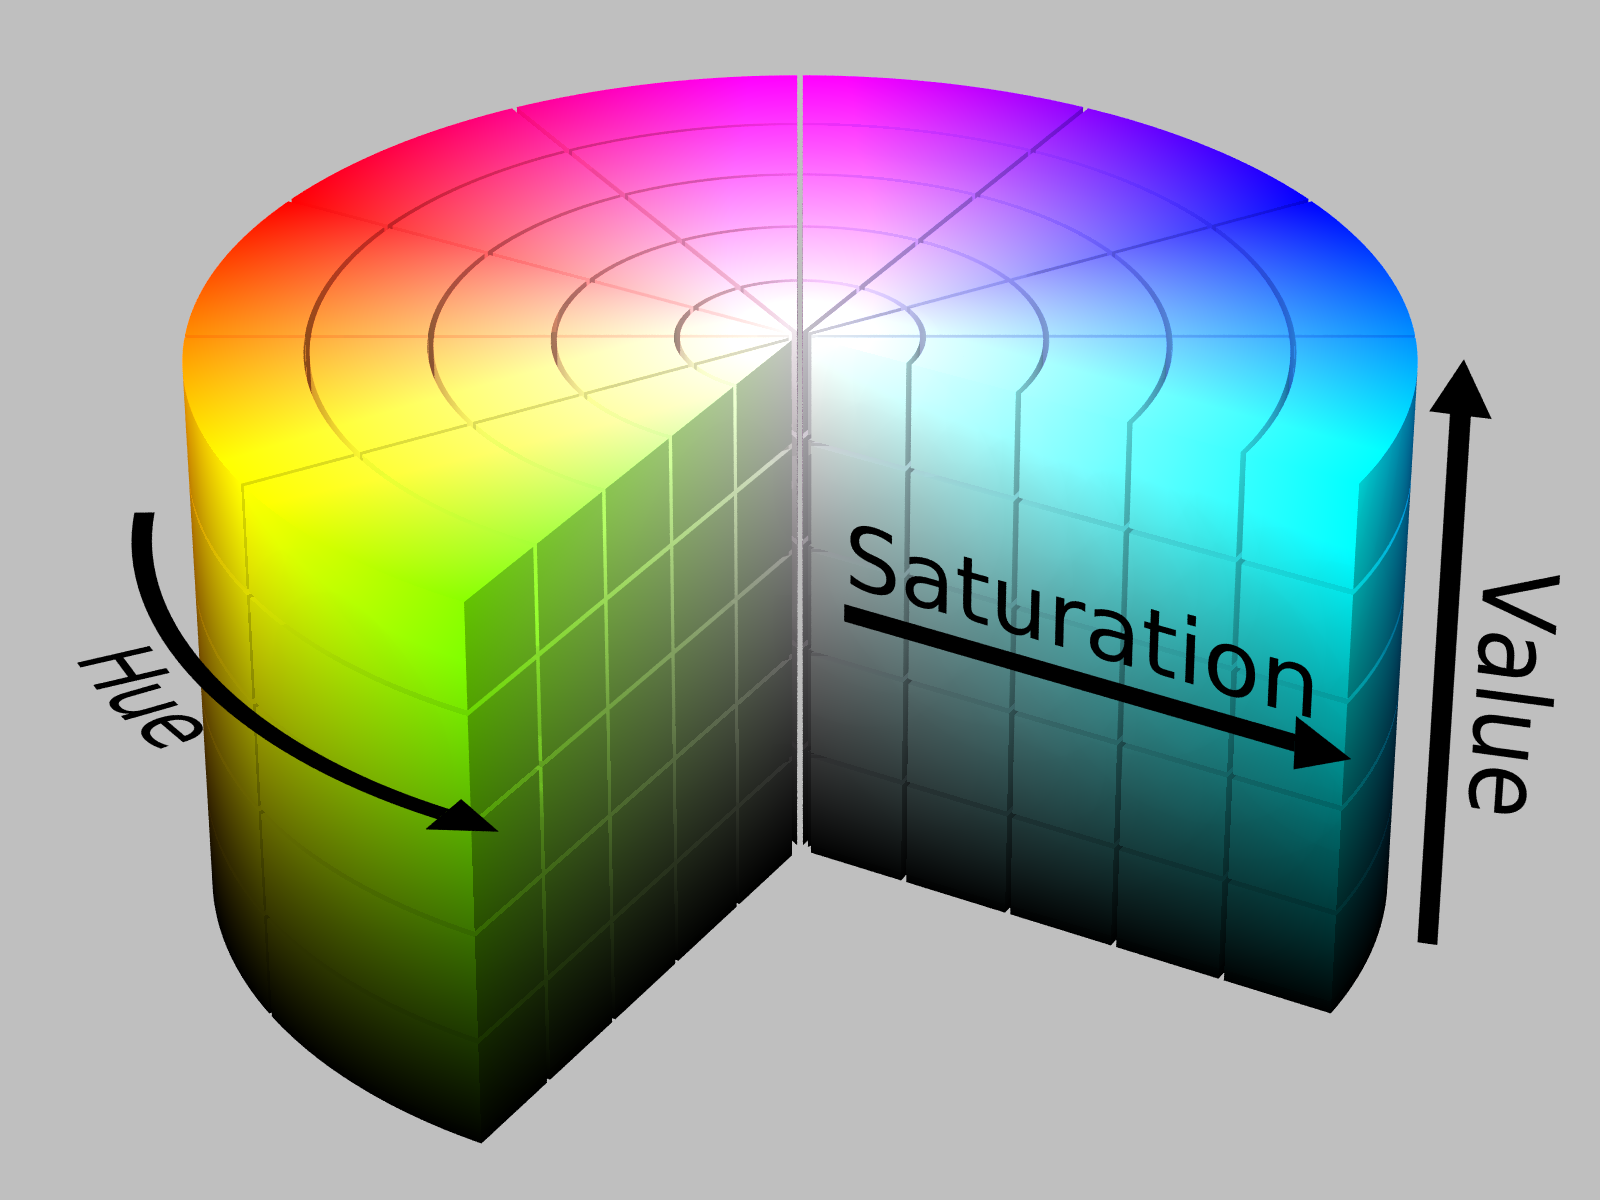
\includegraphics[width=0.7\linewidth]{figures/hsv}
	\caption{HSV Colour Space}
	\label{fig:hsv}
\end{figure}


\subsection{Skin Colour}

Skin detection in HSV tends to be more accurate than RGB. As the colour our Hue in HSV trends to be affected much less be external parameters such as ambient light or direct sunlight.

After careful research a paper found on human skin colour\cite{skinDetection}, in the HSV colour plane, found that the skin colour of the majority of people across the globe lies within the range 6\textsuperscript{o} - 38\textsuperscript{o}. The paper when on to discuss how to continue to improve the reliability of finding skin tones within an image although this is beyond the scope of this project as it would make the functions to be described much more computationally expensive. 
 
\section{Design}
\label{sec:design}
This section will explain how both tasks A and B will be completed, giving diagrams and flowcharts of how the E-Pucks will carry out a particular task.
\subsection{Task A}
To begin designing a solution to the tasks set out in section \ref{sec:intro}, one must first decide upon the different behaviours to be implemented for the tasks. A relatively simple task to be implemented, which would be beneficial to both the first and second task, would be to implement a love behaviour.

Section \ref{sec:background} discussed how each behaviour would perform, illustrating that the love behaviour would follow but not touch the leading object. A second behaviour to be implemented would be an adaption of the aforementioned love behaviour, although instead of the E-Puck following an object it would instead follow a bright light placed before it. The E-Puck would use both the camera to discover any spots of light that have a much higher intensity than its surroundings.

One third and final possible behaviour to implement, providing time permits the group to do so, would be to to implement a obstacle avoidance behaviour. The behaviour which attempts to avoid any nearby objects whilst moving in a particular direction. When it approaches an object it changes its direction to move away from the object.

The first and final behaviours rely heavily on the infrared senses situated on around the edge of the E-Puck. The E-Puck will read in from the infrared sensors, each returning a voltage reading to the chip. This reading can then be used within a formula to calculate the distances to a nearby object. When an object is discovered nearby, the E-Puck must either turn to face it or alter it's direction to move away from it, for the love and obstacle avoidance behaviours respectively. The E-Puck is then required to move forward at a fixed speed until either the object is very close, but not touching for the love behaviour or no longer detected for the hate behaviour.

To create the second behaviour of an attraction to light the E-Puck must be implemented in a similar way to the previously mentioned behaviours, although instead of reading the infrared sensor value for distance one will measure the amount of ambient light falling onto the device.

\subsection{Task B}
Task B requires the group to implement 2 different E-Pucks and cause each to do their own tasks. One E-Puck will be required to follow a hand whilst the other E-Puck will be required to follow the first E-Puck. This may seem similar after implementing the behaviours from task A, although many issues could arise with this task. These issues will be discussed toward the end of this section.

Since the love behaviour will have already been implemented once the implementation of task B begins it would be logical to make use of these behaviours to save time. Therefore to obtain the the desired output of the second E-Puck (the following of the first E-Puck), one may use this behaviour and achieve the required result.

For the first E-Puck, the E-Puck which will be following a human hand, the group will have to use both the camera and infrared sensors on the E-Puck and consult the research performed within section \ref{sec:background} surrounding the colour of human skin.

The E-Puck will begin by discovering any near-by objects using the infra-red sensors before turning the front camera towards any discovered objects. The front camera will then read in the image of the object. Removing a few rows of pixels from the image, for fast processing, the pixels will then be processed to find any required colour that the E-Puck is looking for, the colour of a hand. This processing will be done in the HSV colour plane as to reduce the impact lighting has on the colour of an image.

\subsubsection{Flowchart}
\begin{figure}
	\centering
	\captionsetup[subfigure]{justification=centering}
	\begin{subfigure}{0.45\textwidth}
		\centering
		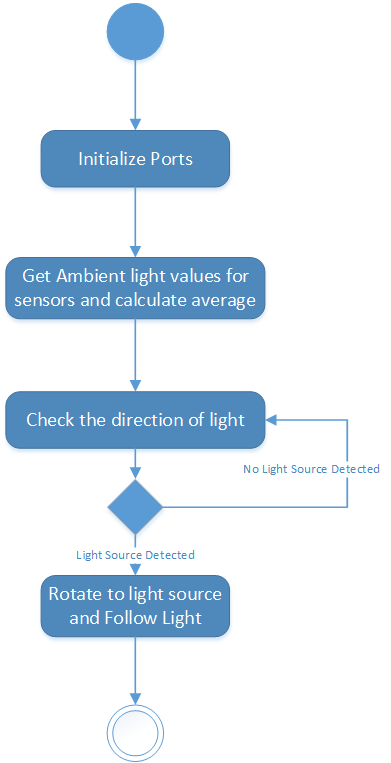
\includegraphics[width=0.5\textwidth]{figures/FollowLight.png}
		\label{fig:flowFollowLight}
		\caption{Flow chart describing \\ the follow light function}
	\end{subfigure}
	\begin{subfigure}{0.45\textwidth}
		\centering
		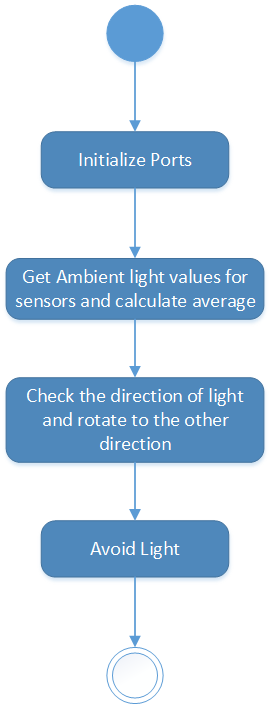
\includegraphics[width=0.5\textwidth]{figures/AvoidLight.png}
		\label{fig:flowAvoidLight}
		\caption{Flow chart describing \\ the avoid light function}
	\end{subfigure}
	\begin{subfigure}{0.9\textwidth}
		\centering
		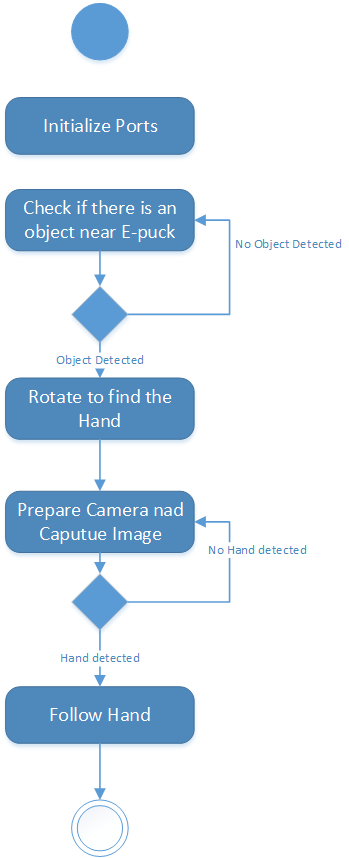
\includegraphics[width=0.3\textwidth]{figures/FollowHand.png}
		\label{fig:flowFollowHand}
		\caption{Flow chart describing \\ the follow hand function}
	\end{subfigure}
\caption{Flow charts describing 3 of the different behaviours implemented within the E-Puck}
\label{fig:flowBehav}
\end{figure}

\begin{figure}
\centering
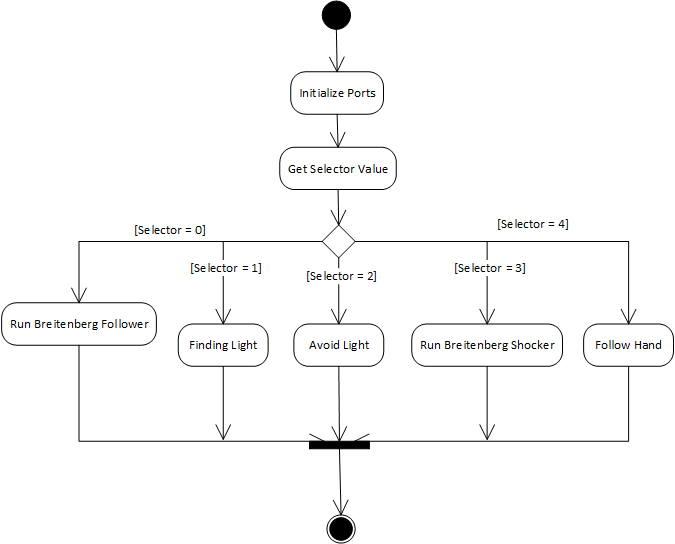
\includegraphics{figures/Main.png}
\caption{Flow chart describing how the main function will be implemented}
\label{fig:flowMain}
\end{figure}

\section{Implementation}
\label{sec:implementation}
This section will describe how each of the tasks mentioned in section \ref{sec:design} have been implemented, explaining the functions within the code, and any discrepancies between the design and final implementation.

The design was gradually implemented in stages, building up to the final completed solution to each task. To make the project easier to implement the demo project provided on the E-Puck\cite{epuck} website was used as a template.
\subsection{Main File}
Within the demo project one can find the main file. This main file starts by finding the position of the selection, a single hexadecimal digit. This selector then decides which function will be called. This becomes very useful to the groups project as then each behaviour needed to be implemented can be ran when a unique selector is selected. Table \ref{table:selectorOptions} clearly shows the possible choices to the user with the code being displayed in the code snippet \ref{code:mainSelector}.

\begin{table}
	\centering
	\begin{tabular}{|c | c|} 
	\hline
	Selector & Function \\ \hline
	0 & run\_breitenberg\_follower \\ \hline
	1 & finding\_light \\ \hline
	2 & avoid\_light \\ \hline
	3 & run\_breitenberg\_shocker \\ \hline
	4 & followHand \\ \hline
	\end{tabular}
	\label{table:selectorOptions}
	\caption{A table to show what function is ran for each selector.}
\end{table}

The functions shown in table \ref{table:selectorOptions} will each be discussed in detail throughout this section.

\begin{lstlisting}[frame=single,caption={Descriptive Caption Text},label=code:mainSelector, float,floatplacement=H]
	selector=getselector();
	if (selector==0) {
		run_breitenberg_follower();
	} else if (selector==1) {
		finding_light();
	} else if (selector==2) {
		avoid_light();
	} else if (selector==3) {
		run_breitenberg_shocker();
	} else if (selector==4) {
		followHand();
	} else{
	}
\end{lstlisting}

\subsection{Breitenburg Follower}
The `run\_breitenburg\_follower' function is a function that was taken from the demo project mentioned previously
\section{Testing \& Results}
\label{sec:ResultsTesting}
This section will first look at the testing that was completed throughout the project to ensure all the processes the were implemented within the E-Puck function as expected. Secondly this section will analyse the results and outcome obtained from running the completed project on the E-Pucks.

\subsection{Testing}
Testing took place throughout the entirety of the implementation stage, before more in-depth testing took place once the implementation had been completed. This testing could be completed in such a way because of the `AGILE' work flow which took place, where the code development would be completed in stages and gradually built up. Therefore each stage can be partially tested after it had been completed.

Firstly, once the main file had been completed, instead of calling the required function, the function name was printed to the terminal. This allowed the group to test if the selector is working properly on the device.

The next heavily tested stage took place when implementing the follow and avoid light functions. This function required careful altering of the variables which set the threshold for finding a nearby light source. This threshold was found using trial and error changing the variable to fit better in all environments as opposed to optimising it for a single environment.

The final function to be tested throughout testing, which also required careful tweaking to complete, was the `followHand' function. Within this function the threshold to evaluate whether the object in front of the camera is a hand or not must be carefully assessed. This was done once again by trial and error, obtaining a the value by improving the last after each test.

One major improvement made because of these tests was that because the image is only taken when an object is found in front of the camera using the infrared sensor much more of the image could be processed and thus finding a hand becomes much more accurate. 

Throughout the final testing of the E-Puck, the E-Puck was ran in a range of scenarios and expected to complete the tasks set out in the introduction of this report. One of the major problems found whilst testing was that the E-Puck would find the hand in front of the camera but then immediately lose track of it again and become stationary. Whilst lowering the threshold for this task solved the problem it also introduced a new one where the E-Puck would follow much more devices not consisting of the colour of human skin

After many different attempts to solve the problem a simple yet effective solution was put into place where once a hand is detected in front of the camera, the E-Puck will then continue to follow the object whilst the object is in range of the infrared sensors. This stops the E-Puck repeatedly taking pictures with the camera and performing costly algorithms on them. This method also greatly reduces battery power and is much more computationally inexpensive for the E-Puck to run.

\subsection{Results}
\label{sec:Results}
Throughout the testing of the software implemented within the E-Puck, analysis of the performance of both E-Pucks were also taken. Each behaviour was found to perform particularly well when running individually. With the E-Pucks performing exactly as expected.

One strange anomaly found whilst testing the E-Puck is that the infrared sensors do not pick up the ambient light produced from a single LED, the flash on a smart phone for example, very well. Whilst this was an issue with the E-Puck itself there was not much the group could do to improve the results in this situation. For all other sources of light, providing they were not too dim, the E-Puck responded very well turning and moving towards the light source.

One other small issue found whilst testing the E-Pucks was with the second E-Puck that was to follow the first. The E-Puck would very often lose track of the first E-Puck, which is possibly down to the speed at which they are traveling with respect to each other. Although, the maneuver where the first E-Puck turns fairly quickly increases the probability of the second E-Puck losing track of it. To try to reduce the frequency that this error occurred the speeds were altered to find an optimum speed at which the 2 E-Pucks operated best together. 

Overall, all of the features preformed very well on the majority of the tests, preforming much better than expected at finding hands with different skin tones and a light source in different lighting environments.
\section{Conclusion}


\clearpage

\appendix
\section{Code}
\subsection{Main}
\subsubsection{C File}
\lstinputlisting{Code/main.c}

\subsection{finding\_Light}
\subsubsection{Header File}
\lstinputlisting{Code/finding_Light.h}
\subsubsection{C File}
\lstinputlisting{Code/finding_Light.c}

\subsection{avoidlight}
\subsubsection{Header File}
\lstinputlisting{Code/avoidlight.h}
\subsubsection{C File}
\lstinputlisting{Code/avoidlight.c}

\subsection{followHand}
\subsubsection{Header File}
\lstinputlisting{Code/followHand.h}
\subsubsection{C File}
\lstinputlisting{Code/followHand.c}

\clearpage 
\bibliography{References}
\bibliographystyle{plain}


\end{document}